\documentclass[11pt,compress,t,notes=noshow, aspectratio=169, xcolor=table]{beamer}

\usepackage{../../style/lmu-lecture}
% Defines macros and environments
% This file is included in slides and exercises

% Rarely used fontstyle for R packages, used only in 
% - forests/slides-forests-benchmark.tex
% - exercises/single-exercises/methods_l_1.Rnw
% - slides/cart/attic/slides_extra_trees.Rnw
\newcommand{\pkg}[1]{{\fontseries{b}\selectfont #1}}

% Spacing helpers, used often (mostly in exercises for \dlz)
\newcommand{\lz}{\vspace{0.5cm}} % vertical space (used often in slides)
\newcommand{\dlz}{\vspace{1cm}}  % double vertical space (used often in exercises, never in slides)
\newcommand{\oneliner}[1] % Oneliner for important statements, used e.g. in iml, algods
{\begin{block}{}\begin{center}\begin{Large}#1\end{Large}\end{center}\end{block}}

% Don't know if this is used or needed, remove?
% textcolor that works in mathmode
% https://tex.stackexchange.com/a/261480
% Used e.g. in forests/slides-forests-bagging.tex
% [...] \textcolor{blue}{\tfrac{1}{M}\sum^M_{m} [...]
% \makeatletter
% \renewcommand*{\@textcolor}[3]{%
%   \protect\leavevmode
%   \begingroup
%     \color#1{#2}#3%
%   \endgroup
% }
% \makeatother


\title{Interpretable Machine Learning}
% \author{LMU}
%\institute{\href{https://compstat-lmu.github.io/lecture_iml/}{compstat-lmu.github.io/lecture\_iml}}
\date{}

\begin{document}
	
	
	% Set style/preamble.Rnw as parent.
	
	% Load all R packages and set up knitr
	
	% This file loads R packages, configures knitr options and sets preamble.Rnw as 
	% parent file
	% IF YOU MODIFY THIS, PLZ ALSO MODIFY setup.Rmd ACCORDINGLY...
	
	% Defines macros and environments
	
	\newcommand{\titlefigure}{figure/counterfactuals_heat.png}
    \newcommand{\learninggoals}{
    	\item See two strategies to generate CEs
    	\item Know problems and limitations of CEs}
	
	\lecturechapter{Methods \& Discussion of CEs}
	\lecture{Interpretable Machine Learning}
	
	% ------------------------------------------------------------------------------


\begin{frame}{Overview of Counterfactual Methods}
Many methods exist to generate counterfactuals, they mainly differ in:
    
	\begin{itemize}[<+->]
		  \item \textbf{Target:} Most support classification; few extend to regression\\
  $\leadsto$ Recent work extends CEs to other ML tasks (un-, semi-, self-supervised)
 \item \textbf{Data type:} Focus is on tabular data; little work on text, vision, audio
		\item \textbf{Feature space:}  Some handle only numerical features; few support mixed types
        %Some methods can only handle numerical features, few can process mixed (numerical and discrete) feature spaces
		\item \textbf{Objectives:} 
        From core goals like sparsity and plausibility to emerging aims such as fairness, personalization, and robustness
        %Many methods focus on action guidance, plausibility and sparsity, few on other objectives like fairness or individual preferences
		\item \textbf{Model access:} 
        Methods range from model-specific (requiring model internals or access to gradients) to model-agnostic (using only prediction functions)
        %Methods either require access to complete model internals, access to gradients, or only to prediction functions \\
        %$\leadsto$ Model-agnostic and model-specific methods exist
		 \item \textbf{Optimization:} 
         From gradient-based (differentiable models) and mixed-integer programming (linear models) to gradient-free methods (e.g., genetic algorithms)
         %From gradient-based (for differentiable models) to gradient-free and heuristic methods (e.g., genetic algorithms, evolutionary strategies)
        %Gradient-based algorithms (only for differentiable models), mixed-integer programming (only linear), or gradient-free algorithms e.g. Nelder-Mead, genetic algorithm
		\item \textbf{Rashomon Effect:} Many methods return one CE, some diverse sets of CEs, others prioritize CEs, or let the user choose
	\end{itemize}
\end{frame}

\begin{frame}{First Optimization Method \citebutton{Wachter et. al (2018)}{http://dx.doi.org/10.2139/ssrn.3063289}}
Introduced counterfactual explanations in the context of ML predictions by solving
		\begin{equation}
			\argmin_{\xv'} \max_{\lambda} \lambda \underbrace{(\fh(\xv') - y')^2}_{o_{target}(\fh(\xv'), y')} + \underbrace{\sum\nolimits_{j = 1}^p |x'_j - x_j|/MAD_j}_{o_{input}(\xv', \xv)}
			%\label{eq:wachter}
		\end{equation}
\begin{itemize}
  \item $MAD_j = \text{med}_{i \in \{1, \dots, n\}} \left( | x^{(i)}_j - \text{med}_{k\in \{1, \dots, n\}} (x^{(k)}_j) | \right)$: Median abs. deviation $x_j$
  \item Optimization alternates: Nelder-Mead minimizes over $\xv'$, then $\lambda$ is increased iteratively until a sufficiently close solution is found
\end{itemize}
    % $MAD_j$ is the median absolute deviation of feature $j$. In each iteration, optimizers like Nelder-Mead solve the equation for $\xv'$ and then $\lambda$ is increased until a sufficiently close solution is found \\[0.2cm]
	
	%\pause
	
	This optimization problem has several shortcomings: 	
	\begin{itemize}%[<+->]
		\item No principled way to set $\lambda$; it is increased manually during optimization %We do not know how to choose $\lambda$ a priori 
		\item Emphasis on $o_{\text{target}}$ dominates early iterations\\%; $o_{input}$ is only minimized once prediction is met
        %Due to the maximization of $\lambda$, we focus primarily on the minimization of $o_{target}$\\
		$\leadsto$ Once $\fh(\xv') \approx y'$ is met, we focus on minimizing $o_{input}$ 
		\item Definition of $o_{input}$ only covers numerical features 
		\item Additional objectives such as sparsity and plausibility are not considered
	\end{itemize}
	


	%\footnote[frame]{Wachter S, Mittelstadt B, Russel C (2017). Counterfactual Explanations Without Opening the Black Box: Automated Decisions and the GDPR. Harvard Journal of Law \& Technology, 31 (2), 2018. \url{http://dx.doi.org/10.2139/ssrn.3063289}}
\end{frame}

\begin{frame}{Multi-Objective CE \citebutton{Dandl et al. (2020)}{https://arxiv.org/abs/2004.11165}}
	\begin{itemize}
		\item \textbf{Multi-Objective Counterfactual Explanations (MOC):} Instead of collapsing objectives into a single objective, optimize all four objectives simultaneously
	$$	\argmin_{\xv'} \left(o_{target}(\fh(\xv'), y'), o_{input}(\xv', \xv), o_{sparse}(\xv', \xv), o_{plausible}(\xv', \Xmat) \right). $$
		
		\item Avoids using/tuning of weights (e.g., \(\lambda\)); returns Pareto-optimal set
        %Note: Weighting parameters like $\lambda$ not necessary anymore
		%\item This approach is called Multi-Objective Counterfactual Explanations (MOC) and was developed by Dandl et al. in 2020. 
		\item Uses an adjusted multi-objective genetic algorithm (NSGA-II) for mixed features %ture types (numeric/categorical)
        %Uses an adjusted multi-objective genetic algorithm (NSGA-II) to produce a set of diverse CEs for mixed discrete and continuous feature spaces
		\item Outputs diverse CEs representing different trade-offs between objectives
        %Instead of one, MOC returns multiple CEs that represent different trade-offs between the objectives and are constructed to be diverse in feature space
	\end{itemize}

	%\footnote[frame]{Dandl et al. (2020) Multi-Objective Counterfactual Explanations. In: Bäck T. et al. (eds) Parallel Problem Solving from Nature – PPSN XVI. PPSN 2020. Lecture Notes in Computer Science, vol 12269. Springer, Cham.}
\end{frame}

\begin{frame}{Example: Credit Data}
	\begin{itemize}
		\item Model: SVM with RBF kernel
		\item $\xv$: First data point of credit data with $\P(y = good)  = 0.34$ %of being a ``good" customer
		\item Goal: Increase the probability to desired outcome $[0.5, 1]$
		\item MOC (with default parameters) returned 69 valid CEs after 200 iterations%found 69 CEs after 200 iterations that met the target
		\item All CEs modified credit duration; many also adjusted credit amount
        %proposed changes to credit duration and many of them to credit amount
	\end{itemize}
\end{frame}

\begin{frame}{Example: Credit Data \citebutton{Dandl et al. (2020)}{https://arxiv.org/abs/2004.11165}}
\begin{itemize}
	\item<1-> Feature changes can be visualized using parallel and 2D surface plots
    %We can visualize feature changes with a parallel plot and 2-dim surface plot
		\item<1-> Parallel plot: All CEs had values equal to or smaller than the values of $\xv$
		\item<2-> Surface plot: CEs in lower-left appear distant, but lie in high-density regions near training data (as shown by histograms)
        %CE why these feature changes are recommended 
		%\item<2-> Counterfactuals in the lower left corner seem to be in a less favorable region far from $\xv$, but they are in high density areas close to training samples (indicated by histograms)
	\end{itemize}
	\begin{columns}[totalwidth=\textwidth]\only<1->{
	\begin{column}{0.5\textwidth}  
	\centering
			%\begin{center}
		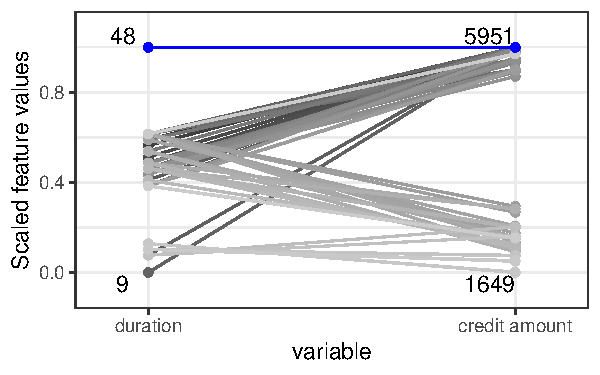
\includegraphics[width=0.75\textwidth]{figure/counterfactuals_credit_parallel}\\
			%\end{center}
		%\vspace{-0.2cm}
			\scriptsize{
            \textbf{Parallel plot:} Grey lines = CEs $\xv'$, blue line = $\xv$. Features without changes omitted. \\
            Bold numbers denote numeric ranges.
            %\textbf{Parallel plot:} Grey lines show feature values of CEs $\xv'$, blue line are values of $\xv$. Features without proposed changes are omitted. Bold numbers refer to range of numeric features.
            } 
			
		\end{column}}
		\visible<2->{
		\begin{column}{0.5\textwidth}
			%\begin{center}
			\centering
			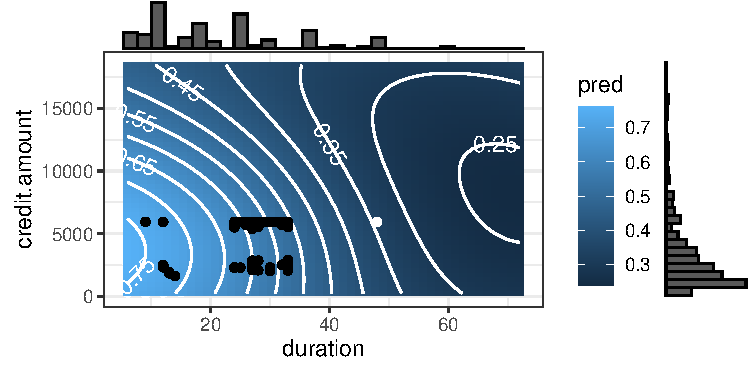
\includegraphics[width=\textwidth]{figure/counterfactuals_credit_heat}\\
			%\end{center}
		%\vspace{-0.2cm}
			\scriptsize{
            \textbf{Surface plot:} 
            White dot = $\xv$, black dots = CEs $\xv'$.
            %White dot is $\xv$, black dots are CEs $\xv'$. \\
			\textbf{Histograms:} Marginal distribution of training data $\Xmat$.
            } 
		\end{column}
		}
	\end{columns}
%\footnote[frame]{Dandl S., Molnar C., Binder M., Bischl B. (2020) Multi-Objective Counterfactual Explanations. In: Bäck T. et al. (eds) Parallel Problem Solving from Nature – PPSN XVI. PPSN 2020. Lecture Notes in Computer Science, vol 12269. Springer, Cham.}
\end{frame}


%\begin{frame}{Example: Bike Sharing Dataset}
%	\begin{itemize}
%		\item Model: Random Forest with 500 trees
%		\item $\xv$ is the first data point of the dataset with $\fh(\xv) = 1767.93$ rental bikes. 
%		\item Our desired goal is to increase the count of total rental bikes to $y' = [3000, \infty[$
%		\item MOC (with default parameters) found 56 counterfactuals after 200 iterations that met the target.
%		\item Most counterfactuals proposed to decrease the humidity (94.6 \%) and more than half to increase the temperature (55.4\%). 
%		\item Some counterfactuals proposed additional changes to the year (2012 instead of 2011) and month (December instead of Januar).
%		\framebreak 
%		\item We can visualize feature changes with a parallel plot. 
%		\item For humidity and temperature, we can additionally show a 2-dim surface plot. 
%	\end{itemize}
%	\vspace{-0.5cm}
%	\begin{columns}[totalwidth=\textwidth]
%		\begin{column}{0.5\textwidth}
%			\begin{center}
%				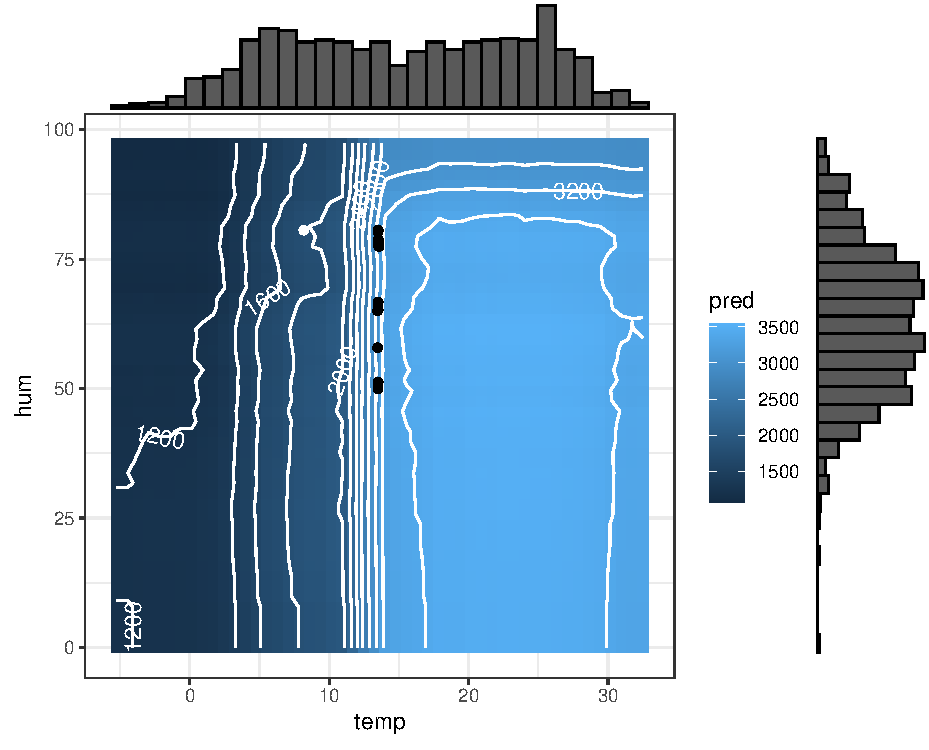
\includegraphics[width=1\textwidth]{figure/counterfactuals_bike_sp}
%			\end{center}
%		
%			\scriptsize{\textbf{Figure:} Response surface plot. 
%				The white dot is $\xv$, black dots are $\xv'$. The histograms display the marginal distribution of the training data $\Xmat$.} 
%				
%		\end{column}
%		\begin{column}{0.5\textwidth}  
%			\begin{center}
%				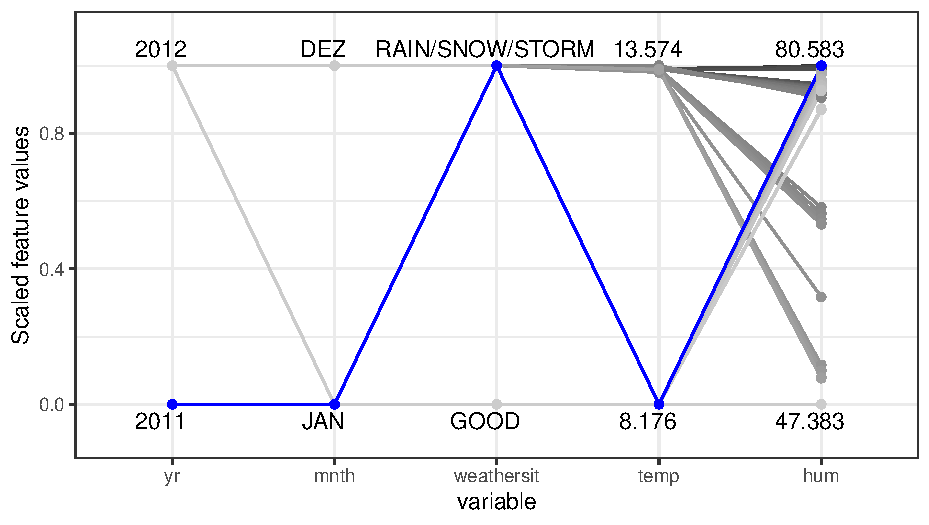
\includegraphics[width=1\textwidth]{figure/counterfactuals_bike_para}
%			\end{center}
%		
%		\scriptsize{\textbf{Figure:} Parallel plot. 
%			The grey lines show the feature values of the counterfactuals $\xv'$, the blue line corresponds to the values of $\xv$. Features without proposed changes are omitted. The bold numbers give minima and minima of numeric features while character strings indicate categories of character features.} 
%		
%		\end{column}
%	\end{columns}
%\end{frame}

\begin{frame}{Problems, Pitfalls, \& Limitations}
\begin{itemize}[<+->]
    \item \textbf{Illusion of model understanding:} 
    CEs explain ML decisions by pointing to few specific alternatives, reducing complexity but offering limited explanatory power\\
    $\leadsto$ %psychologists showed that even though the perceived model-understanding of end-users increases, the objective model-understanding remained unchanged
    Psychologists have shown that although perceived model understanding of end-users increases, the objective model understanding remains unchanged
    
    %\item \textbf{Finding the right metric:} Similarity is the crucial concept for finding good CEs. However, our concept of similarity is context and domain dependent. E.g. while L1 can be a reasonable notion for tabular data, it is counterintuitive for image data. Sparsity is often desirable for end-users but not for data scientists searching for biases in the model.
    \item \textbf{Right metric:} Similarity measures are crucial to find good CEs (depends on context/domain)\\
    $\leadsto$ e.g., $L_1$ can be reasonable for tabular data but not for image data\\
    $\leadsto$ sparsity desirable for end-users but not for auditors searching for model bias

    %\item \textbf{Confusing Model and Real-World:} Explanations of the model do not easily transfer to the process in which a model is applied. This information should be conveyed to the end-user.
    \item \textbf{Confusing Model and Real-World:} Model explanations are not easily transferable to reality\\
    $\leadsto$ End-users must know that CEs provide insights into a model, not real world %models are only approximations %This information should be conveyed to the end-user
    \item \textbf{Disclosing too much information:} 
    CEs can reveal too much information about the model and help potential attackers
    \end{itemize}
\end{frame}

\begin{frame}{Problems, Pitfalls, \& Limitations}
\begin{itemize}[<+->]
    \item \textbf{Rashomon effect:} One, few, all? Which CEs should be shown to the end-user?\\
    $\leadsto$ No universal answer; depends on user goals, cognitive load, and resources
    %No perfect answer, depends on end-users, computational resources, and knowledge
    % \item \textbf{Actionability vs. fairness:} Some authors suggest to focus only on the actionability of CEs\\
    % $\leadsto$ Counteract contestability, e.g., if ethnicity is not changed in a CE since it is not actionable, this could hide racial biases in the model
    \item \textbf{Actionability vs. fairness:} Focus on actionable changes hinder contestability\\
$\leadsto$ E.g., if ethnicity is not changed in a CE since it is not actionable, this could hide racial biases in the model

    \item \textbf{Assumption of constant model:} To provide guidance for the future, CEs assume that their underlying model does not change in the future\\
    $\leadsto$ in reality this assumption is often violated and CEs are not reliable anymore 
    \item \textbf{Attacking CEs:} Researchers can create models with great performance, which generate arbitrary explanations specified by the ML developer\\
    $\leadsto$ how faithful are CEs to the models underlying mechanism?
\end{itemize}

%	\textbf{Pitfall 3:} Rashomon Effect
%	\begin{itemize}
%		\item Due to the Rashomon Effect, multiple counterfactual explanations could be found for an instance. 
%		\item If all counterfactuals are reported the user could be overwhelmed. Instead of a comprehensible explanations for a prediction, users received an even more complex explanations.
%		\item Another option is to only report the ``best" ones. But this requires a notion for ``superiority".  
%		\item Furthermore, users might not be interested in the ``best" but most ``diverse" counterfactuals.
%		\item The best option might be to report all counterfactuals but let the user decide which one to select, e.g., based on their previous knowledge. 
%	\end{itemize}
%	\textbf{Pitfall 4:} 
%	\begin{itemize}
%		\item 
%	\end{itemize}
%	\textbf{Pitfall 5:} Confusing model explanation with real data process explanations
%	\begin{itemize}
%		\item Causal dependencies
%		\item Fixed model at time $t$ 
%		\item Wrong input by user
%	\end{itemize}
\end{frame}

\endlecture
\end{document}
